\documentclass[10pt]{article}

%% PACKAGES
\usepackage{geometry}
 \geometry{ a4paper,
 			total={170mm,257mm},
 			left=20mm,
 			top=20mm}
% temporary version with space for commenting
%\geometry{ 	a4paper,
%			total={140mm,257mm},
%			left=20mm,
%			top=20mm}

\usepackage{authblk}
\usepackage[ruled,vlined]{algorithm2e}

\usepackage[english]{babel}
\usepackage[utf8]{inputenc}
\usepackage[colorlinks=true,
			urlcolor=black,
			linkcolor=black,
			citecolor=black]{hyperref}
\usepackage{amsmath, amsthm, amssymb, mathtools}
\usepackage{listings}
\usepackage{graphicx, color, xcolor}
\usepackage{tabularx}
\usepackage{xspace} %list of punctuation marks 
\usepackage{soul} %strike through text

\usepackage[colorinlistoftodos, textwidth = 40mm]{todonotes}

\usepackage{tikz}
\usetikzlibrary{arrows, positioning, automata}	
\tikzstyle{process} = [	rectangle,
						minimum width=1cm, 
						minimum height=0.8cm,
						text centered, 
						%fill=red!30
						draw=black,]
\tikzstyle{arrow} =[thick,->,>=stealth]

\newtheorem{definition}{Definition}[section]

\newcounter{protocol}
\newenvironment{protocol}[1]
  {\par\addvspace{\topsep}
   \noindent
   \tabularx{\linewidth}{@{} X @{}}
    \hline
    \refstepcounter{protocol}\textbf{Protocol \theprotocol} #1 \\
    \hline}
  { \\
    \hline
   \endtabularx
   \par\addvspace{\topsep}}

% Mathbb
\newcommand{\G}{\ensuremath{\mathbb{G}}\xspace}
\newcommand{\F}{\ensuremath{\mathbb{F}}}
\newcommand{\N}{\ensuremath{\mathbb{N}}\xspace}
\newcommand{\Z}{\ensuremath{\mathbb{Z}}\xspace}

% Mathcal
\newcommand{\receiver}{\ensuremath{\mathcal{R}}\xspace}
\newcommand{\sender}{\ensuremath{\mathcal{S}}\xspace}
\newcommand{\nullifiertree}{\ensuremath{\mathcal{X}}\xspace}
\newcommand{\notetree}{\ensuremath{\mathcal{N}}\xspace}

% Others
%\newcommand{\NoteB}{\ensuremath{N_{B}}\xspace}
%\newcommand{\NoteB}{\ensuremath{N_{A\to B}}\xspace}
%\newcommand{\NoteC}{\ensuremath{N_{C}}\xspace}
%\newcommand{\NoteC}{\ensuremath{N_{B\to C}}\xspace}
\newcommand{\noi}{\noindent}

% Comments
\newcommand{\js}{\todo[size=\small, color=blue!40]}
\newcommand{\jsi}{\todo[inline, size=\small, color=blue!40]}
\newcommand{\xs}{\todo[size=\small, color=green!40]}
\newcommand{\xsi}{\todo[inline, size=\small, color=green!40]}
\newcommand{\mb}{\todo[size=\small, color=red!40]}
\newcommand{\mbi}{\todo[inline, size=\small, color=red!40]}

% mathsf
\newcommand{\klic}{\mathsf{k_{lic}}}
\newcommand{\kreq}{\mathsf{k_{req}}}
\newcommand{\kdh}{\mathsf{k_{DH}}}
\newcommand{\ksym}{\mathsf{k}}
\newcommand{\tkdh}{\mathsf{\tilde{k}_{DH}}}
\newcommand{\tklic}{\mathsf{\tilde{k}_{lic}}}
\newcommand{\tkreq}{\mathsf{\tilde{k}_{req}}}
\newcommand{\sk}{\mathsf{sk}}
\newcommand{\pk}{\mathsf{pk}}
\newcommand{\ck}{\mathsf{ck}}
\renewcommand{\pk}{\mathsf{pk}}
\newcommand{\vk}{\mathsf{vk}}
\newcommand{\npk}{\mathsf{npk}}
\newcommand{\user}{\mathsf{user}}
\newcommand{\NFT}{\mathsf{NFT}}
\newcommand{\LP}{\mathsf{LP}}
\newcommand{\SP}{\mathsf{SP}}
\newcommand{\npkn}[1]{\mathsf{npk}_{#1}}
\newcommand{\nsk}{\mathsf{nsk}}
\newcommand{\lsk}{\mathsf{lsk}}
\newcommand{\lpk}{\mathsf{lpk}}
\newcommand{\rpk}{\mathsf{rpk}}
\newcommand{\spk}{\mathsf{spk}}
\newcommand{\tx}{\mathsf{tx}}
\newcommand{\txold}{\mathsf{tx^{old}}}
\newcommand{\txm}{\mathsf{tx_{metadata}}}
\newcommand{\txp}{\mathsf{tx_{payload}}}
\newcommand{\txh}{\mathsf{tx_{hash}}}
\newcommand{\txproof}{\mathsf{tx_{proof}}}
\newcommand{\Note}{\mathsf{N}}
\newcommand{\lic}{\mathsf{lic}}
\newcommand{\req}{\mathsf{req}}
\newcommand{\Session}{\mathsf{session}}
\newcommand{\SessionCookie}{\mathsf{sc}}
\newcommand{\nfthash}{\mathsf{hash_{NFT}}}
\newcommand{\nftpayload}{\mathsf{payload_{NFT}}}
\newcommand{\sig}{\mathsf{sig}}
\newcommand{\lsig}{\mathsf{sig_{lic}}}
\newcommand{\tsig}{\mathsf{sig_{tx}}}
\newcommand{\attr}{\mathsf{attr}}
\newcommand{\attrhash}{\mathsf{attr\_hash}}
\newcommand{\attrdata}{\mathsf{attr\_data}}
\newcommand{\sign}{\mathsf{sign\_single\_key}}
\newcommand{\signd}{\mathsf{sign\_double\_key}}
\newcommand{\verify}{\mathsf{verify\_sig\_single\_key}}
\newcommand{\verifyd}{\mathsf{verify\_sig\_double\_key}}
\newcommand{\mintnft}{\mathsf{mint\_nft}}
\newcommand{\NoteB}{\mathsf{N_{B}}}
\newcommand{\NoteC}{\mathsf{N_{C}}}
\newcommand{\nnew}[1]{\mathsf{N^{new}_{#1}}}
\newcommand{\nold}[1]{\mathsf{N^{old}_{#1}}}
\newcommand{\vnew}[1]{\mathsf{v_{#1}}}
\newcommand{\vold}[1]{\mathsf{w_{#1}}}
\newcommand{\change}{\mathsf{change}}
\newcommand{\type}{\mathsf{type}}
\newcommand{\com}{\mathsf{com}}
\newcommand{\enc}{\mathsf{enc}}
\newcommand{\Enc}{\mathsf{Enc}}
\newcommand{\nonce}{\mathsf{nonce}}
\newcommand{\pos}{\mathsf{pos}}
\newcommand{\nullifier}{\mathsf{nullifier}}
\newcommand{\isseen}{\mathsf{is\_seen}}
\newcommand{\pnullifiers}{\mathsf{previous\_nullifiers}}
\newcommand{\sessionid}{\mathsf{session\_id}}
\newcommand{\hb}{H^\mathsf{BLAKE2b}}
\newcommand{\hp}{H^\mathsf{Poseidon}}

    
\title{Citadel Protocol Specification}
\date{\today}

\author{Dusk}


\begin{document}

\maketitle

\tableofcontents
\pagebreak 

\section{General Overview}
\label{sec:overview}
% !TeX root = ../build/main.tex

Citadel is a self-sovereign identity (SSI) protocol built on tope of Dusk that allows users of a given service to manage their digital identities in a fully transparent manner. More specifically, every user can know which information about them is shared with other parties, and accept or deny any request for personal information.

\subsection{Properties}

With Citadel, users of a service can request licenses that represent their \emph{right} to use such a service. Citadel satisfies the following properties:

\begin{itemize}
	\item \emph{Proof of ownership}: users can prove that they own a valid license that allows them to use a certain service.
	\item \emph{Proof of validity}: users with a valid license can prove that their license has not been revoked and is valid.
	\item \emph{Unlinkability}: different services used by a same user cannot be linked from one another.
	\item \emph{Decentralized session opening}: when users start using a service, the network learns that this happened and the license used to access to the service cannot be used again.
	\item \emph{Attribute blinding}: users have the power to decide exactly what information they want to share and with whom.
\end{itemize}

\subsection{The parties involved}

Citadel involves three (potentially different) parties:

\begin{itemize}
    \item The \emph{user} is the person who interacts with the wallet and requests licenses in order to claim their right to make use of services.
    \item The \emph{service provider} (SP) is the entity that offers a service to users. Upon verification that a service request from a user is correct, it provides such service.
    \item The \emph{license provider} (LP) is the entity that receives requests for licenses from users, and upon acceptance, issues them. The LP can be the same SP entity or a different one.
\end{itemize}

\subsection{The elements involved}

Below there is the list of the elements involved in the protocol. The details of their structure and their role are explained in the following sections. 

\begin{itemize}
	\item A \emph{request} is a set of information that the user sends to the network in order to inform the LP that they are requesting a license. It includes an stealth address where the license will be sent to.
	\item A \emph{license} is an asset that represents the right of a user to use a certain service. In particular, a license contains a set of attributes that are associated to the requirements needed to make use of that service.
	\item The \emph{LicenseProverParameters} are the set of parameters needed by the user to compute a proof that proves their license ownership.
	\item A \emph{session} is a set of public values sent by the user to the network that are associated with the initiation of the use of a service.
	\item A \emph{session cookie} is a set of values that allows the SP to verify that a session was opened correctly.
\end{itemize}

\subsection{Protocol flow}

{\color{red}[Missing explanation]}

\begin{figure}[h]
	\centering
	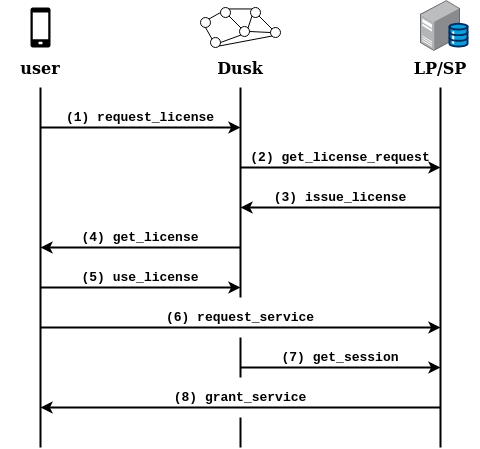
\includegraphics[width=.4\textwidth]{\figs/protocol.png}
	\caption{Overview of the protocol messages exchanged between the user, Dusk's network, and the LP/SP.}
	\label{fig:protocol}
\end{figure}



\section{Definitions}
\label{sec:definitions}
\subsection{The Roles involved} 

\begin{itemize}
    \item \textbf{User:} An entity that interacts with the wallet to request licenses and prove ownership of those.
    \item \textbf{Service Provider:} An entity offering an off-chain service that receives requests for licenses, and upon acceptance, issues them. It also provides the service upon verification that a service request is correct.
\end{itemize}

\subsection{The Elements involved} 

\begin{itemize}
    \item \textbf{Request:} A request includes the encryption of a stealth address belonging to the user, where the license has to be sent to. The structure is as follows:

    \begin{center}
        \begin{tabular}{ |c|c|c|c| } 
        \hline
        \textbf{Element} & \textbf{Type} & \textbf{Info.} \\
        \hline
        $\nonce$ & - & It is a randomness needed to compute $\enc$. \\ 
        $\enc$ & - & It is a ciphertext of size 3. \\
        $(\rpk, R)$ & - & It is a stealth address of the SP. \\
        \hline
        \end{tabular}
    \end{center}


    \item \textbf{License:} A license is an asset that represents the right of a user to use a given service. The structure is as follows:

    \begin{center}
        \begin{tabular}{ |c|c|c|c| } 
        \hline
        \textbf{Element} & \textbf{Type} & \textbf{Info.} \\
        \hline
        $\pos$ & - & It is the position of the license into a Merkle tree of licenses. \\ 
        $\nonce$ & - & It is a randomness needed to compute $\enc$. \\ 
        $\enc$ & - & It is a ciphertext of size 4. \\
        $(\lpk, R)$ & - & It is a stealth address of the user. \\
        \hline
        \end{tabular}
    \end{center}

    \item \textbf{LicenseProverParameters:} A prover needs some auxiliary parameters to compute the proof that nullifies a license when desired to be spent. The structure is as follows:

    \begin{center}
        \begin{tabular}{ |c|c|c|c| } 
        \hline
        \textbf{Element} & \textbf{Type} & \textbf{Info.} \\
        \hline
        $\lpk'$ & - & The license public key prime.\\ 
        $\lsig$ & - & The signature of the license. \\ 
        $\com_0^{hash}$ & - & A hash commitment of the public key of the SP. \\ 
        $\com_1$ & - & A Pedersen Commitment of the attributes. \\ 
        $\com_2$ & - & A Pedersen Commitment of the $c$ value. \\ 
        $\mathsf{tx\_hash}$ & - & The hash of the transaction calling the nullifying contract. \\ 
        $\mathsf{sig}_\mathsf{tx}$ & - & The signature of the transaction calling the nullifying contract. \\ 
        $\mathsf{nullifier}_\mathsf{lic}$ & - & The nullifier of the license. \\ 
        $\mathsf{merkle\_proof}$ & - & Membership proof of the license in the Merkle tree of licenses. \\ 

        \hline
        \end{tabular}
    \end{center}

    \item \textbf{Session Cookie:} A session cookie is a secret value known only by the user and the SP. It contains a set of openings to a given set of commitments. The structure is as follows:

    \begin{center}
        \begin{tabular}{ |c|c|c|c| } 
        \hline
        \textbf{Element} & \textbf{Type} & \textbf{Info.} \\
        \hline
        $\pk_{\SP}$ & - & The public key of the SP. \\ 
        $\attr$ & - & The attributes of the user. \\ 
        $c$ & - & The challenge value. \\ 
        $(\mathsf{s_0}, \mathsf{s_1}, \mathsf{s_2})$ & - & The randomness used to compute the commitments. \\

        \hline
        \end{tabular}
    \end{center}

\end{itemize}

\section{Protocol Workflow}
\label{sec:protocol}
% !TeX root = ../build/main.tex

\mbi{Change BLAKE2 to Poseidon and leave a footnote.}

In this section, we describe the workflow of Citadel in detail.

\begin{enumerate}

\item (\textbf{user}) $\mathsf{request\_license}()$

	\begin{enumerate}
	
		\item Compute a license stealth address $(\lpk, R_{\lic})$ belonging to the user, using the user's own public key, as follows.
			
			\begin{enumerate}
				\item Sample $r$ uniformly at random from $\F_t$.
				\item Compute a symmetric Diffie--Hellman key $\ksym = rA_{\user}$.
				\item Compute a one-time public key $\lpk = \hb(\ksym)G + B_{\user}$.
				\item Compute $R_{\lic} = rG$.
			\end{enumerate}
		
		\item Compute the license secret key $\lsk = \hb(\ksym) + b_{\user}$ and an additional key $\klic = \hp(\lsk)G$. 
		
		\item Compute the request stealth address $(\rpk, R_{\req})$ using the LP's public key, as follows.
			
			\mbi{Consider using different letter instead of $r$...}
			\begin{enumerate}
				\item Sample $r$ uniformly at random from $\F_t$.
				\item Compute a symmetric Diffie--Hellman key $\kreq = rA_{\LP}$.
				\item Compute a one-time public key $\rpk = \hb(\kreq)G + B_{\LP}$.
				\item Compute $R_{\req} = rG$.
			\end{enumerate}
		
		\item Encrypt data using the key $\kreq$: $\enc = \Enc_{\kreq} ((\lpk, R_{\lic})||\klic; \nonce).$
		
			\mbi{Include how the nonce is computed, if it is a random value as well.}
		
		\item Send the following request to the network: $\req = ((\rpk, R_{\req}), \enc, \nonce).$
		
	\end{enumerate}


\item (\textbf{LP}) $\mathsf{get\_license\_request()}$

	The LP checks continuously the network to detect any incoming license requests addressed to them:
	
	\begin{enumerate}
		\item Compute $\tkreq = a_{\LP}R_{\req}$.
		\item Check if $\rpk \stackrel{?}{=} \hb(\tkreq) G + B_{\LP}$.
	\end{enumerate}

\item (\textbf{LP}) $\mathsf{issue\_license()}$
	
	\begin{enumerate}
		\item Upon receiving a request from a user, define a set of attributes $\attr$ representing the license, and compute a digital signature as follows:
				$$\lsig = \sign_{\sk_{\SP}}(\lpk, \attr).$$
		\item Encrypt the signature and the attributes using the license key:
			  	$$\enc = \Enc_{\klic} (\lsig || \attr; \nonce).$$
		\item Send the following license to the network:
				$$\lic = ((\lpk, R_{\lic}), \enc, \nonce, \pos).$$
	\end{enumerate}
	
\item (\textbf{user}) $\mathsf{get\_license()}$

	In order to receive the license, the user must scan all incoming transactions the following way:
	
	\begin{enumerate}
		\item Compute $\tklic = \hb(\lsk)G$.
		\item Check if $\lpk \stackrel{?}{=} \hb(\tklic) G + B_{\user}$, 
	\end{enumerate}	
	
\item (\textbf{user}) $\mathsf{use\_license()}$

	When using the license, open a session with a specific SP by executing a call to the license contract. The following steps are performed:
	
	\mbi{We should mention something about the license contract before this step. Maybe in Section 2 where elements are presented? Add a small section about Dusk's blockchain?}
	%or something like: the actions performed by the user are interactions with a wallet software, etc. (add part of Milosz' explanation there - or leave it to implementation details).
	%discuss this with Xavi.
	
	\begin{itemize}
		\item The user issues a transaction that calls the license contract, which includes a ZKP that is computed out of the gadget depicted in Figure \ref{fig:circuit_prove_nft}. Notice that here, the user signs $\mathsf{session\_hash}$ using $\lsk$. Likewise, the user here will need to compute $\lpk' = \lsk G'$.
		\item The network validators will execute the smart contract, which verifies the proof. Upon success, the following session will be added to a shared list of sessions:
		
		$$\Session = \{\mathsf{session\_hash}, \sessionid, \com_0^{hash}, \com_1, \com_2\},$$
		
		where $\mathsf{session\_hash} = \hp(\pk_{\SP} || r_\mathsf{session})$, and $r_\mathsf{session}$ is sampled uniformly at random from $\F_t$.
		
		
	\end{itemize}
	
\item (\textbf{user}) $\mathsf{request\_service()}$

Request the service to the SP, establishing communication using a secure channel, and providing the session cookie that follows.
	
	$$\SessionCookie = \{\pk_{\mathsf{SP}}, r_\mathsf{session}, \sessionid, \pk_{\LP}, \attr, c, \mathsf{s_0}, \mathsf{s_1}, \mathsf{s_2}\}$$
	
\item (\textbf{SSP}) $\mathsf{get\_session()}$

Receive a $\Session$ from the list of sessions, where $\Session.\sessionid = \SessionCookie.\sessionid$.
	
\item (\textbf{SSP}) $\mathsf{grant\_service()}$

Grant or deny the service upon verification of the following steps:
	
	\begin{itemize}
		\item Check whether the values $(\attr, \pk_{\LP}, c)$ included in the $\SessionCookie$ are correct.
		\item Check whether the opening $(\pk_{\SP}, r_\mathsf{session})$ included in the $\SessionCookie$ matches the $\mathsf{session\_hash}$ found in the $\Session$.
		\item Check whether the openings $((\pk_{\LP}, \mathsf{s_0}), (\attr, \mathsf{s_1}), (c, \mathsf{s_2}))$ included in the $\SessionCookie$ match the\\
			  commitments ($\com_0^{hash}, \com_1, \com_2$) found in the $\Session$.
	\end{itemize}

\end{enumerate}
	
%\begin{figure}[h]
%	\centering
%	\setlength{\fboxsep}{5pt}%
%	\setlength{\fboxrule}{0.3pt}%
%	\fbox{
%		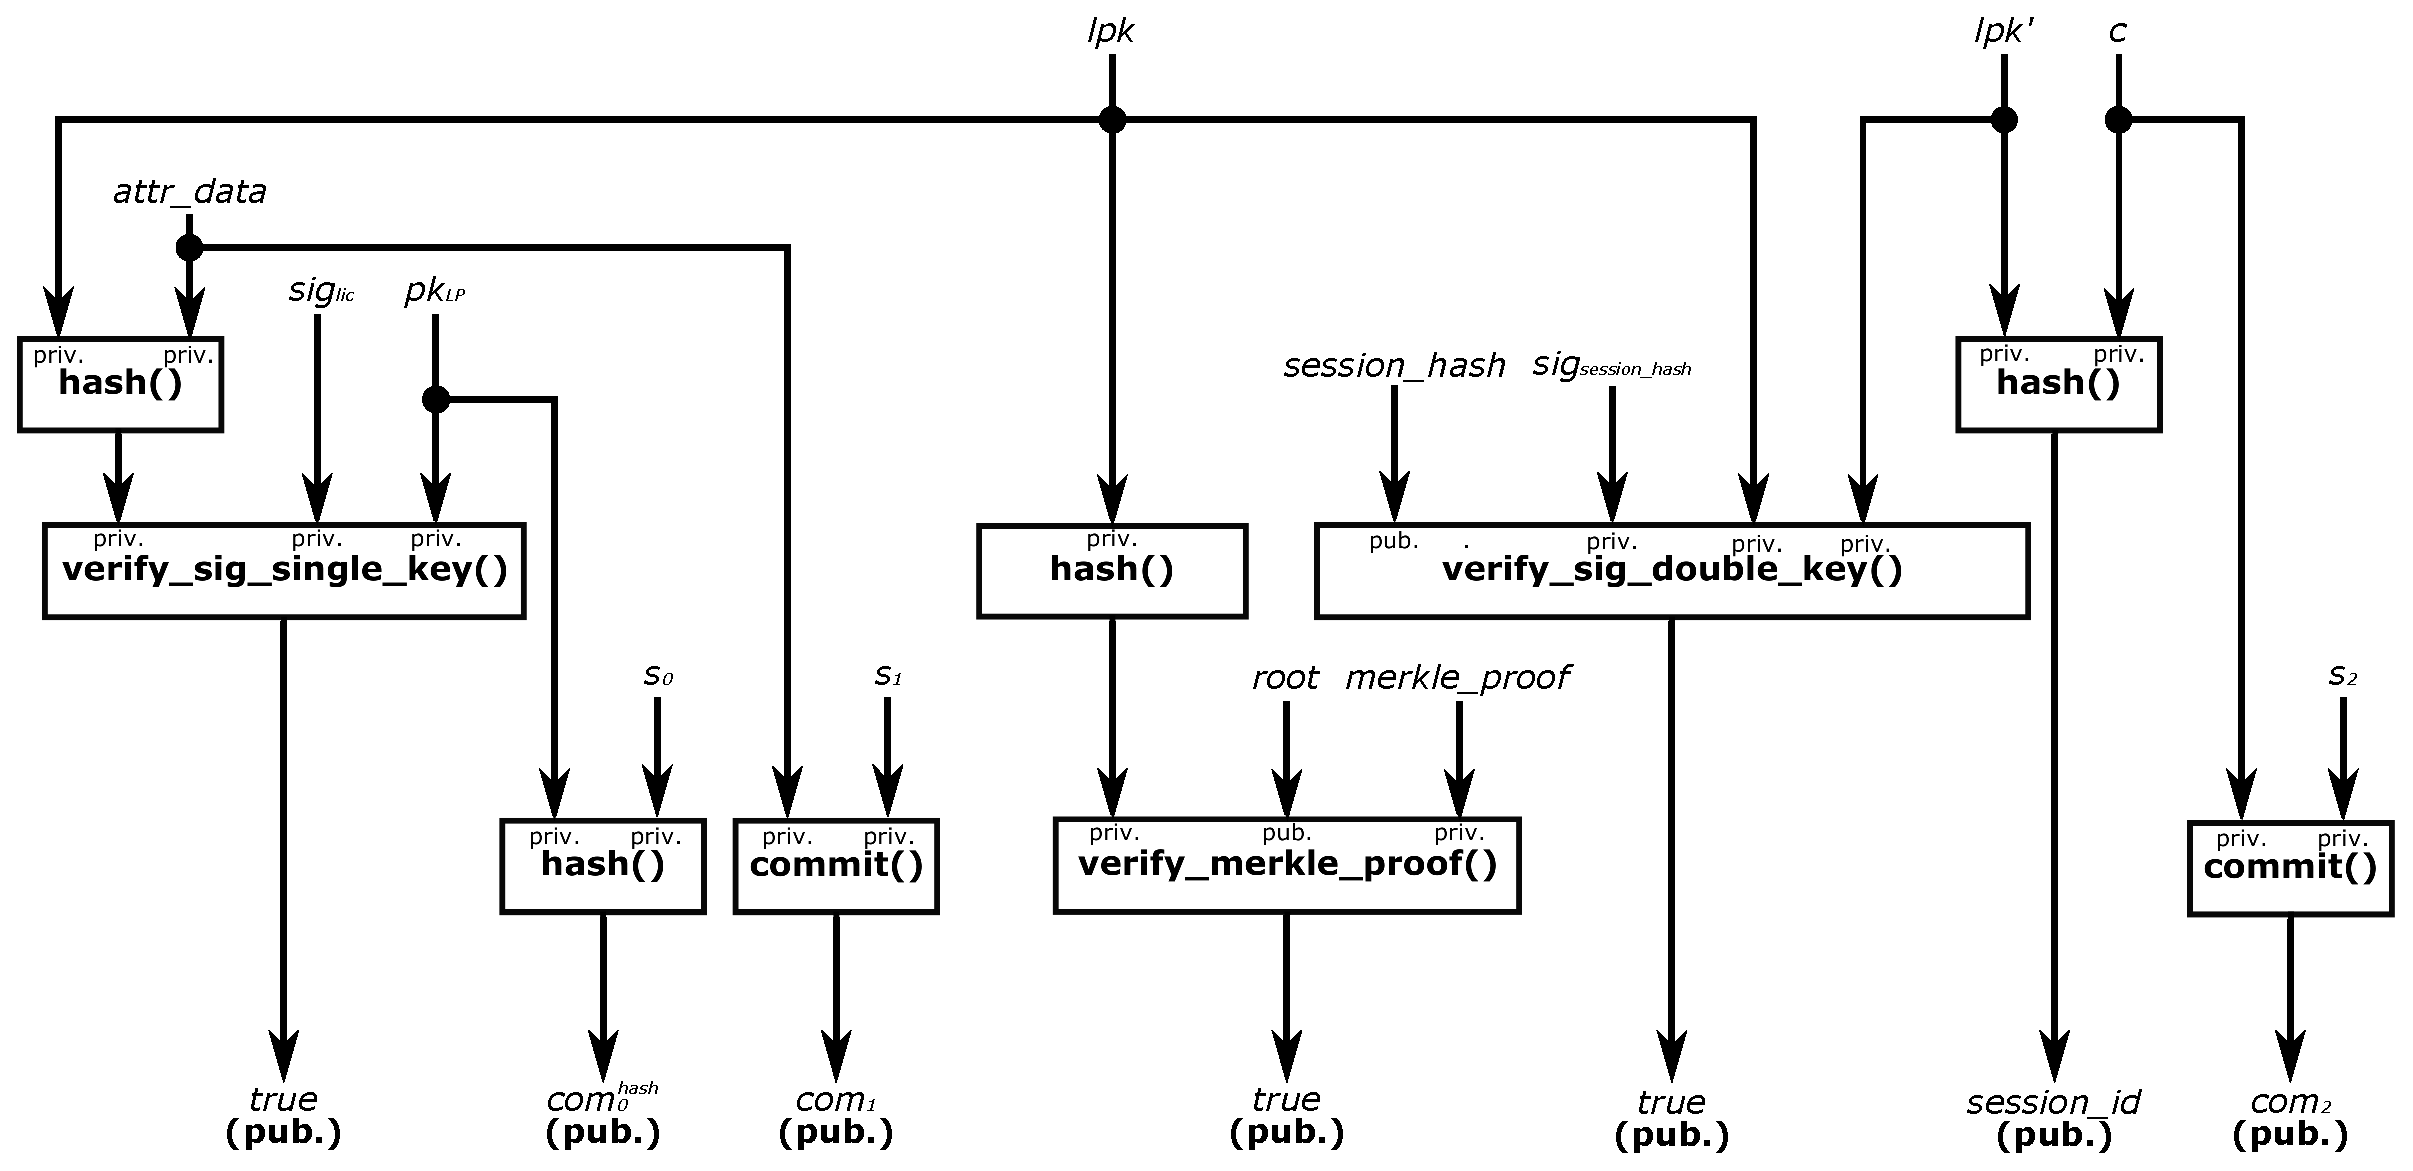
\includegraphics[width=460pt,draft=false]{images/circuit_prove_nft.eps}}
%	\caption{Arithmetic circuit for proving a license's ownership.}
%	\label{fig:circuit_prove_nft}
%\end{figure}

Furthermore, the SP might want to prevent the user from using the license more than once (e.g. this is a single-use license, like entering a concert). This is done through the computation of $\sessionid$. The deployment of this part of the circuit has two different possibilities:
\begin{itemize}
	\item If we set $c = 0$ (or directly remove this input from the circuit), the license can be used only once.
	\item If the SP requests the user to set a custom value for $c$ (e.g. the date of an event), the license can be reused only under certain conditions.
\end{itemize}



\section{Protocol Implementation}
\label{sec:implementation}

\subsection{Participants} 
Protocol implementation involves realization of the protocol building blocks as well as providing means of data communication between them. Building blocks are placed at the following locations, which correspond to protocol participants:

\begin{itemize}%[label=$\bullet$]
	\item User software.
	\item License Provider software.
	\item Service Provider software.
	\item License contract.
\end{itemize}

\begin{flushleft}
Data communication between protocol participants is realized in the following modes:
\end{flushleft}

\begin{itemize}%[label=$\bullet$]
	\item Calling a contract state changing method.
	\item Calling a contract state querying method (not modifying the contract state).
	\item Storing data directly in blockchain.
	\item Retrieving data from blockchain.
	\item Delegating ZK proof calculation.
	\item Calling off-chain.
\end{itemize}

\begin{flushleft}
The following diagram illustrates an interaction between protocol participants and indicates the communication means used.
\end{flushleft}

\begin{figure}[h]
	\centering
		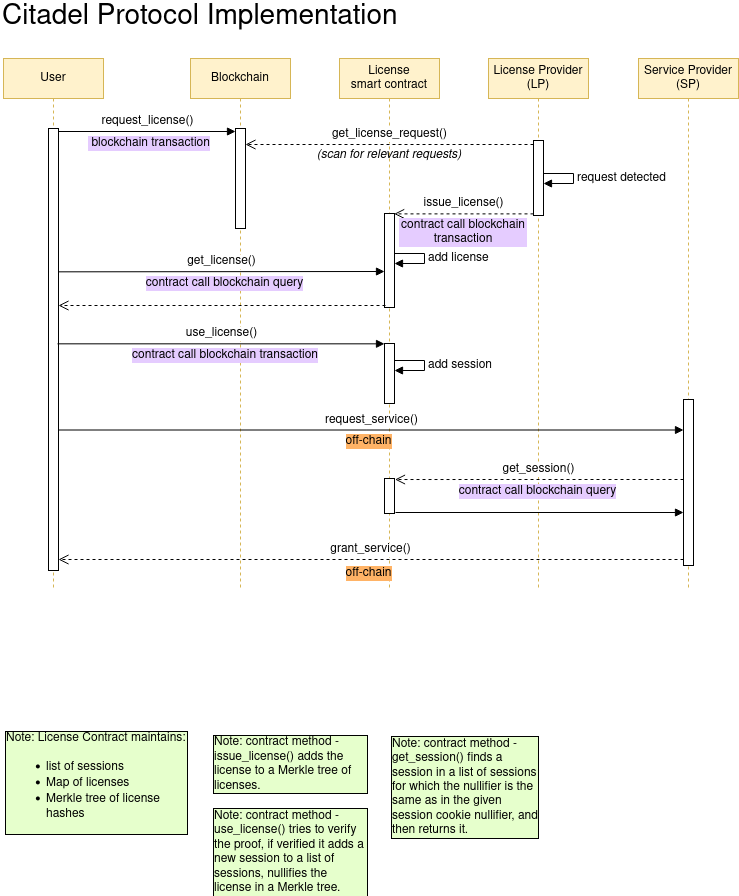
\includegraphics[width=390pt,draft=false]{images/implementation.png}
	\caption{Interaction between protocol participants}
	\label{fig:implementation}
\end{figure}

\begin{flushleft}
On the diagram, we can see various communication modes being used. Initially, the user submits to the blockchain a transaction which contains request as a payload. Subsequently, the License Provider, which continuously scans the blockchain, detects transactions containing requests and filters out requests which are addressed to it. The License Provider can obtain requests via other routes as well, for example via http or email, passing requests on the blockchain is only one of many possible ways of submitting a request, one that has the advantage of passing a payment along with the request. Once the License Provider gets a hold of a request, it can perform appropriate verification, and upon successful verification, it can issue a license. Issuing a license involves a smart contract transaction call. Smart contract transaction call is a blockchain transaction, yet to not confuse the reader, we show it on the diagram with details of blockchain involvement omitted. The user obtains licenses via a contract query. For privacy reasons, the user obtains a bulk of licenses not pertaining exclusively to her and filters it out by herself. To economize the volume of data transfers, block-height range is passed to allow for tranfer of a subset of available records. All modes of communication used so far were on-chain. Communication between the user and the Service Provider, on the other hand, is off-chain. When the Service Provider wants to establish a session, it calls a contract to obtain a session for the given session id.
\end{flushleft}

The diagram illustrates the following flow of data and interactions between participants:

\begin{itemize}%[label=$\bullet$]
	\item User submits request to a License Provider by issuing a blockchain transaction.
	\item License Provider scans the blockchain and obtains the request.
	\item License Provider, upon necessary verification, issues a license.
	\item License Provider sends license to the License Contract via a smart contract call transaction.
	\item User obtains licenses for a given block-height range.
	\item User filters out licenses addressed to her/him.
	\item User calculates a proof (the proof calculation might be delegated).
	\item User calls \textit{use-license} to redeem a license, via a smart contract call.
	\item License Contract attempts to verify the proof and, if verified, adds a new session to a list of sessions.
	\item User requests a service from a Service Provider (off-chain).
	\item Service Provider asks contract for a session.
	\item Service Provider grants service to the user (off-chain).
\end{itemize}


\subsection{License Contract}

\begin{flushleft}
License contract maintains state consisting of the following data:
\end{flushleft}

\begin{itemize}%[label=$\bullet$]
	\item List of sessions.
	\item Map of licenses and their positions in the Merkle tree.
	\item Merkle tree of license hashes.
\end{itemize}


\begin{flushleft}
Contract provides the following methods:
\end{flushleft}

\begin{itemize}%[label=$\bullet$]
	\item \textit{issue-license}: adds a license to a Merkle tree of licenses.
	\item \textit{get-licenses}: provides a list of new licenses added in a given block-height range.
	\item \textit{use-license}: attempts to verify the proof and, if verified, adds a new session to a list of sessions and nullifies the license in the Merkle tree.
	\item \textit{get-session}: finds a session in a list of sessions and returns it to the caller.
\end{itemize}


\subsection{License ZK Proof Calculation}

License ZK proof calculation will either be performed by the user or delegated to a node. At the time of writing, the details of delegation are not yet known, they will be filled in here once the information becomes available.


\end{document}













